\documentclass[11pt,a4paper]{article}

% ---------- Packages ----------
\usepackage[a4paper,margin=2.4cm]{geometry}
\usepackage{amsmath,amssymb,mathtools}
\usepackage{physics}
\usepackage{xcolor}
\usepackage{tcolorbox}
\tcbuselibrary{skins,breakable}
\usepackage{enumitem}
\usepackage{fancyhdr}
\usepackage{titlesec}
\usepackage{listings}
\usepackage{hyperref}
\usepackage{lastpage}
\usepackage{booktabs}
\usepackage{array}
\usepackage{graphicx}
\usepackage{microtype}
\usepackage{bookmark}

% ---------- NIT Calicut Palette & Theme Colours ----------
\definecolor{ntccblue}{RGB}{20,60,110}       % #143C6E Deep Navy
\definecolor{ntccgold}{RGB}{175,130,20}      % Amber Gold
\definecolor{boxgrey}{RGB}{245,245,248}
\definecolor{keybg}{RGB}{235,242,250}
\definecolor{probbg}{RGB}{250,244,230}
\definecolor{pitbg}{RGB}{252,235,238}
\definecolor{histbg}{RGB}{238,248,235}
\definecolor{expbg}{RGB}{240,247,250}
\definecolor{solbg}{RGB}{248,250,252}

% Code listing colours
\definecolor{codegreen}{rgb}{0,0.6,0}
\definecolor{codegray}{rgb}{0.5,0.5,0.5}
\definecolor{codepurple}{rgb}{0.58,0,0.82}
\definecolor{backcolour}{rgb}{0.96,0.96,0.94}

\lstdefinestyle{mystyle}{
    backgroundcolor=\color{backcolour},
    commentstyle=\color{codegreen},
    keywordstyle=\color{ntccblue}\bfseries,
    numberstyle=\tiny\color{codegray},
    stringstyle=\color{codepurple},
    basicstyle=\ttfamily\footnotesize,
    breakatwhitespace=false,
    breaklines=true,
    captionpos=b,
    keepspaces=true,
    numbers=left,
    numbersep=6pt,
    showspaces=false,
    showstringspaces=false,
    showtabs=false,
    tabsize=2,
    frame=single,
    rulecolor=\color{black!15}
}
\lstset{style=mystyle}

% ---------- Hyperref Setup ----------
\hypersetup{
    colorlinks=true,
    linkcolor=ntccblue,
    citecolor=ntccblue,
    urlcolor=ntccblue,
    pdftitle={Module 1: Crystal Physics and Reciprocal Lattice - Student Copy},
    pdfauthor={Department of Physics, National Institute of Technology Calicut}
}

% ---------- Section Styling ----------
\titleformat{\section}
  {\normalfont\Large\bfseries\color{ntccblue}}
  {\thesection}{0.6em}{}[{\color{ntccgold}\titlerule[1.2pt]}]
\titleformat{\subsection}
  {\normalfont\large\bfseries\color{ntccblue}}
  {\thesubsection}{0.6em}{}
\titleformat{\subsubsection}
  {\normalfont\bfseries\color{black}}
  {\thesubsubsection}{0.6em}{}

% ---------- Header & Footer ----------
\pagestyle{fancy}
\fancyhf{}
\renewcommand{\headrulewidth}{0.4pt}
\fancyhead[L]{\small\itshape PH7302E -- Condensed Matter Physics}
\fancyhead[R]{\small\itshape Module 1: Crystal Physics \& Reciprocal Lattice}
\fancyfoot[C]{\small \thepage\ of \pageref{LastPage}}

% ---------- tcolorbox Environments ----------
\newtcolorbox{keybox}[1][Key Concept]{
  colback=keybg, colframe=ntccblue, boxrule=0.6pt, arc=2pt,
  left=8pt, right=8pt, top=6pt, bottom=6pt,
  title={#1}, fonttitle=\bfseries\small, coltitle=white,
  colbacktitle=ntccblue, boxsep=2pt, breakable
}

\newtcolorbox{physbox}[1][Physical Picture]{
  colback=boxgrey, colframe=ntccblue!60!black, boxrule=0.5pt, arc=2pt,
  left=8pt, right=8pt, top=6pt, bottom=6pt,
  title={#1}, fonttitle=\bfseries\small, coltitle=white,
  colbacktitle=ntccblue!60!black, boxsep=2pt, breakable
}

\newtcolorbox{probbox}[1][Tutorial / Practice Problem]{
  colback=probbg, colframe=ntccgold!85!black, boxrule=0.6pt, arc=2pt,
  left=8pt, right=8pt, top=6pt, bottom=6pt,
  title={#1}, fonttitle=\bfseries\small, coltitle=white,
  colbacktitle=ntccgold!85!black, boxsep=2pt, breakable
}

\newtcolorbox{solbox}[1][Worked Example \& Solution]{
  colback=solbg, colframe=ntccblue!70, boxrule=0.6pt, arc=2pt,
  left=8pt, right=8pt, top=6pt, bottom=6pt,
  title={$\blacktriangleright$~#1}, fonttitle=\bfseries\small, coltitle=white,
  colbacktitle=ntccblue!70, boxsep=2pt, breakable
}

\newtcolorbox{pitbox}[1][Pitfall \& Common Misconception]{
  colback=pitbg, colframe=red!65!black, boxrule=0.6pt, arc=2pt,
  left=8pt, right=8pt, top=6pt, bottom=6pt,
  title={\textbf{!}~#1}, fonttitle=\bfseries\small, coltitle=white,
  colbacktitle=red!65!black, boxsep=2pt, breakable
}

\newtcolorbox{takebox}[1][Take-home Summary]{
  colback=keybg, colframe=ntccgold, boxrule=0.8pt, arc=3pt,
  left=8pt, right=8pt, top=6pt, bottom=6pt,
  title={$\bigstar$~#1}, fonttitle=\bfseries\small, coltitle=black,
  colbacktitle=ntccgold, boxsep=2pt, breakable
}

\begin{document}

% ==================== TITLE PAGE / HEADER ====================
\begin{center}
    {\large \textsc{National Institute of Technology Calicut}}\\[0.2cm]
    {\large \textbf{Department of Physics}}\\[0.3cm]
    {\huge \bfseries \color{ntccblue} PH7302E: Condensed Matter Physics}\\[0.25cm]
    {\Large \bfseries \color{ntccgold} Module 1: Crystal Physics \& Reciprocal Lattice}\\[0.2cm]
    {\normalsize \textbf{Comprehensive Student Lecture Guide \& Tutorial Companion}}\\[0.2cm]
    {\small Academic Year 2026--2027 \quad$\vert$\quad Instructor: Course Faculty}
\end{center}
\vspace{0.2cm}
\hrule height 1.2pt
\vspace{0.5cm}

\tableofcontents
\newpage

% ==================== PREFACE & OUTCOMES ====================
\section*{Instructions to the Student}
\addcontentsline{toc}{section}{Instructions to the Student}

This document is the official \textbf{Student Edition} for \textbf{Module 1: Crystal Physics and Reciprocal Lattice} of the postgraduate core course \emph{PH7302E: Condensed Matter Physics} at the National Institute of Technology Calicut. 

\begin{keybox}[Structure of This Guide]
\begin{itemize}[leftmargin=1.5em]
    \item \textbf{Consolidated Assignment 1:} Contains all 24 required tutorial problems upfront with numerical answer hints to guide your independent problem solving.
    \item \textbf{In-Depth Lecture Modules:} Four master lectures covering Crystal Systems, Miller Indices, Reciprocal Lattices, Diffraction Physics, Symmetry, and Structure Factors.
    \item \textbf{Integrated Worked Examples (\texttt{solbox}):} Detailed step-by-step mathematical proofs and physical calculations placed directly alongside the theoretical concepts.
    \item \textbf{Publication-Grade Vector Visualizations:} 6 custom vector illustrations detailing 3D unit cells, Wigner-Seitz cells, Miller planes, Bragg \& Ewald diffraction geometry, Brillouin zones, and BCC destructive extinctions.
    \item \textbf{Computational Python Demonstrations:} Minimal, reproducible Python scripts for computing reciprocal lattices, indexing powder patterns, and simulating diffraction geometry.
\end{itemize}
\end{keybox}

\section*{Learning Outcomes}
\addcontentsline{toc}{section}{Learning Outcomes}

Upon rigorous study of this module and completion of Assignment 1, you will be able to:
\begin{enumerate}[leftmargin=1.8em, label=\bfseries LO\arabic*:]
    \item Distinguish rigorously between mathematical lattices, physical bases, primitive cells, and conventional unit cells.
    \item Classify crystals systematically into the 7 crystal systems and 14 three-dimensional Bravais lattices.
    \item Calculate indices for crystal directions $[uvw]$ and planes $(hkl)$, and evaluate interplanar spacings $d_{hkl}$.
    \item Derive primitive reciprocal vectors $\mathbf{b}_i$, construct the first Brillouin zone, and establish the reciprocal duality between BCC and FCC lattices.
    \item Formulate the Bragg condition and Laue diffraction condition ($\Delta\mathbf{k} = \mathbf{G}$), and geometrically interpret diffraction via the Ewald sphere.
    \item Calculate geometric structure factors $F_{hkl}$ for multi-atom bases (BCC, FCC, Diamond, Zinc Blende, NaCl, CsCl) and identify systematic extinction rules.
    \item Master experimental diffraction techniques (Laue, Rotating Crystal, Powder XRD) and index cubic diffraction patterns.
    \item Analyze crystallographic point groups, space groups, and apply \emph{Neumann's Principle} to explain tensor properties such as dielectric response and piezoelectricity.
\end{enumerate}

\newpage

% ==================== ASSIGNMENT 1 ====================
\section*{Assignment 1: Crystal Physics \& Reciprocal Lattice}
\addcontentsline{toc}{section}{Assignment 1: Crystal Physics \& Reciprocal Lattice}

\begin{probbox}[Submission Guidelines]
Complete all 24 problems below. Write clear, step-by-step derivations with labeled diagrams and explicit units. Submit your completed solutions before the Mid-Semester Examination deadline. Answer hints are provided in brackets to guide your verification.
\end{probbox}

\subsection*{Lecture 1: Crystal Geometry \& Miller Indices}
\begin{enumerate}[leftmargin=1.8em, label=\textbf{1.\arabic*}]
    \item Show that the maximum sphere packing fraction of a Face-Centered Cubic (FCC) lattice is $\frac{\pi}{3\sqrt{2}} \approx 0.74$. \hfill \textbf{[Hint: $4r = a\sqrt{2}$, 4 atoms/cell, $\eta \approx 74.05\%$]}
    \item How many atoms are contained within the conventional unit cell of the diamond cubic lattice? Explain the contribution from the underlying Bravais lattice and the basis. \hfill \textbf{[Hint: $4 \text{ points} \times 2 \text{ atoms} = 8\text{ atoms}$]}
    \item Sketch the $(110)$ plane in a BCC conventional unit cell and identify all corner and body-centered atoms lying exactly on this plane. \hfill \textbf{[Hint: Cuts opposite edges; contains 2 corners and 1 center atom]}
    \item A crystal plane intercepts the crystallographic axes at $2a$, $3b$, and $6c$. Determine its Miller indices $(hkl)$. \hfill \textbf{[Hint: Intercepts $(2,3,6) \implies (\frac{1}{2}, \frac{1}{3}, \frac{1}{6}) \implies (321)$]}
    \item Calculate the interplanar spacing $d_{220}$ for copper, which crystallizes in FCC with lattice constant $a = 3.61\,\text{\AA}$. \hfill \textbf{[Hint: $d_{220} = \frac{3.61}{\sqrt{8}} = 1.276\,\text{\AA}$]}
    \item Sketch the $(11\bar{2})$ plane within a cubic unit cell, clearly indicating the choice of origin and negative axis intercept. \hfill \textbf{[Hint: Intercepts at $x=1$, $y=1$, $z=-1/2$]}
\end{enumerate}

\subsection*{Lecture 2: Reciprocal Lattices \& Diffraction Conditions}
\begin{enumerate}[leftmargin=1.8em, label=\textbf{2.\arabic*}]
    \setcounter{enumi}{6}
    \item Derive the primitive reciprocal lattice vectors for a two-dimensional hexagonal direct lattice with $\mathbf{a}_1 = a(1,0)$ and $\mathbf{a}_2 = a(1/2, \sqrt{3}/2)$. Show that the reciprocal lattice is also hexagonal. \hfill \textbf{[Hint: Enclose angle of $60^\circ$ or $120^\circ$, magnitude $\frac{4\pi}{\sqrt{3}a}$]}
    \item Starting from the primitive translation vectors of a BCC lattice, prove that its reciprocal lattice is Face-Centered Cubic (FCC) with conventional cubic side $4\pi/a$. \hfill \textbf{[Hint: $V = a^3/2$, $\mathbf{b}_1 = \frac{2\pi}{a}(\hat{y}+\hat{z})$]}
    \item Prove rigorously that the reciprocal lattice vector $\mathbf{G}_{hkl} = h\mathbf{b}_1 + k\mathbf{b}_2 + l\mathbf{b}_3$ is perpendicular to the direct lattice plane family $(hkl)$, and that the interplanar spacing is $d_{hkl} = 2\pi/|\mathbf{G}_{hkl}|$. \hfill \textbf{[Hint: Evaluate $\mathbf{G}\cdot(\frac{\mathbf{a}_1}{h}-\frac{\mathbf{a}_2}{k}) = 0$]}
    \item Calculate the Bragg glancing angle $\theta$ and detector angle $2\theta$ for the $(200)$ reflection in NaCl ($a = 5.64\,\text{\AA}$) using Cu K$\alpha$ radiation ($\lambda = 1.54\,\text{\AA}$). \hfill \textbf{[Hint: $d_{200} = 2.82\,\text{\AA} \implies \theta \approx 15.84^\circ, 2\theta \approx 31.68^\circ$]}
    \item Show that, among the FCC-allowed reflections of the diamond structure, the structure factor vanishes identically whenever $h+k+l = 4n+2$ ($n \in \mathbb{Z}$). \hfill \textbf{[Hint: Phase factor $e^{i\pi(4n+2)/2} = e^{i\pi(2n+1)} = -1$]}
    \item Explain from first principles of wave interference why the $(100)$ diffraction peak is forbidden in a BCC crystal but fully allowed in a Simple Cubic crystal. \hfill \textbf{[Hint: Path difference to body center is $\lambda/2 \implies$ phase difference $\pi$]}
\end{enumerate}

\subsection*{Lecture 3: Experimental Methods \& Crystal Symmetry}
\begin{enumerate}[leftmargin=1.8em, label=\textbf{3.\arabic*}]
    \setcounter{enumi}{12}
    \item Index the first five diffraction lines of a Debye-Scherrer powder pattern obtained from BCC $\alpha$-iron ($a = 2.87\,\text{\AA}$) using Cu K$\alpha$ radiation ($\lambda = 1.54\,\text{\AA}$). Calculate their respective $2\theta$ values. \hfill \textbf{[Hint: $(110), (200), (211), (220), (310)$; $2\theta = 44.6^\circ, 64.9^\circ, 82.2^\circ, 98.7^\circ, 116.1^\circ$]}
    \item Explain why the powder diffraction method produces sharp diffraction peaks even though individual microcrystallites in the sample are randomly oriented. \hfill \textbf{[Hint: Formation of continuous Debye-Scherrer cones around the incident beam]}
    \item Determine the multiplicity factor $p$ for the $\{110\}$ family of planes in a cubic crystal system. List all 12 planes explicitly. \hfill \textbf{[Hint: 6 pairs of opposite faces $\implies p = 12$]}
    \item Prove the Crystallographic Restriction Theorem: show that a five-fold rotational axis ($C_5$) is mathematically incompatible with 2D or 3D translational periodicity. \hfill \textbf{[Hint: $2\cos\phi = m \implies \cos(72^\circ) = \frac{\sqrt{5}-1}{4} \notin \frac{\mathbb{Z}}{2}$]}
    \item Identify the full point-group symmetry of an ideal cube in both Schoenflies ($O_h$) and Hermann-Mauguin ($m\bar{3}m$) notations. How many symmetry operations does it possess? \hfill \textbf{[Hint: 48 operations: 24 proper rotations + inversion]}
    \item How many distinct plane crystallographic (wallpaper) groups exist in two dimensions, and how many Bravais lattices span them? \hfill \textbf{[Hint: 17 wallpaper groups spanning 5 2D Bravais lattices]}
\end{enumerate}

\subsection*{Lecture 4: Quantitative Structure Factors \& Advanced Applications}
\begin{enumerate}[leftmargin=1.8em, label=\textbf{4.\arabic*}]
    \setcounter{enumi}{18}
    \item Metallic copper has an FCC structure with lattice constant $a = 3.61\,\text{\AA}$ and atomic weight $M = 63.55\,\text{g/mol}$.
    \begin{enumerate}[label=(\alph*)]
        \item Calculate the metallic atomic radius $r_{\text{Cu}}$. \hfill \textbf{[Hint: $r = a\sqrt{2}/4 = 1.276\,\text{\AA}$]}
        \item Calculate the theoretical mass density $\rho_{\text{Cu}}$ in $\text{g/cm}^3$. \hfill \textbf{[Hint: $\rho = \frac{4 \times 63.55}{N_A a^3} \approx 8.93\,\text{g/cm}^3$]}
        \item Calculate the interplanar spacing $d_{111}$. \hfill \textbf{[Hint: $d_{111} = 3.61/\sqrt{3} = 2.084\,\text{\AA}$]}
    \end{enumerate}
    \item The first-order Bragg diffraction from $(110)$ planes of a BCC crystal is observed at $2\theta = 30.0^\circ$ using monochromatic X-rays of wavelength $\lambda = 1.54\,\text{\AA}$. Determine the crystal lattice constant $a$. \hfill \textbf{[Hint: $\theta = 15^\circ \implies d = 2.975\,\text{\AA} \implies a = d\sqrt{2} = 4.207\,\text{\AA}$]}
    \item Using direct matrix inversion or reciprocal projection, show that the reciprocal lattice of a direct 2D hexagonal lattice with angle $60^\circ$ is also hexagonal, but rotated by $30^\circ$ relative to the direct lattice. \hfill \textbf{[Hint: Encloses angle of $60^\circ$; rotated axes]}
    \item Polycrystalline sodium (BCC) is examined by XRD with $\lambda = 1.54\,\text{\AA}$. The first diffraction ring is observed at $2\theta = 29.8^\circ$. Identify the reflecting plane and determine the cubic lattice parameter $a_{\text{Na}}$. \hfill \textbf{[Hint: First BCC reflection is $(110) \implies \theta = 14.9^\circ \implies a \approx 4.236\,\text{\AA}$]}
    \item Derive the structure factor for the Zinc Blende (ZnS) crystal structure. Explain why the $(200)$ reflection, which is completely extinct in silicon/diamond, has a non-zero observable intensity in GaAs. \hfill \textbf{[Hint: $F_{200} = 4(f_{\text{Ga}} - f_{\text{As}}) \neq 0$ because $f_{\text{Ga}} \neq f_{\text{As}}$]}
    \item Formulate Neumann's Principle for physical property tensors. Explain why centrosymmetric crystals cannot exhibit piezoelectricity, whereas non-centrosymmetric crystals (e.g. quartz, zinc blende) can. \hfill \textbf{[Hint: Piezoelectric tensor $d_{ijk}$ is 3rd rank; changes sign under inversion]}
\end{enumerate}

\newpage

% ==================== LECTURE 1 ====================
\section{Lecture 1: Crystal Structure Basics \& Miller Indices}

\subsection{PART A: Crystal Structure Basics}

\subsubsection{1.1 Introduction to Condensed Matter Physics}
Condensed matter physics investigates how macroscopic material properties emerge from microscopic electromagnetic interactions among vast ensembles ($\sim 10^{23}$) of electrons and atomic nuclei. A central paradigm of modern solid-state physics is the deep relationship between structural symmetry in real space and electronic, thermal, and optical behavior.

\begin{keybox}[Fundamental Paradigm of Crystal Physics]
$$\text{Crystal Structure} = \text{Lattice} + \text{Basis}$$
\begin{itemize}[leftmargin=1.5em]
    \item \textbf{Lattice:} A purely mathematical, periodic infinite array of discrete points in space.
    \item \textbf{Basis:} A physical motif of one or more atoms identically placed relative to each lattice point.
\end{itemize}
\end{keybox}

\subsubsection{1.2 Mathematical Lattices, Primitive Cells, and Wigner-Seitz Construction}
An ideal three-dimensional crystal lattice is invariant under any translation of the form:
\begin{equation}
\mathbf{R} = n_1\mathbf{a}_1 + n_2\mathbf{a}_2 + n_3\mathbf{a}_3, \qquad n_1, n_2, n_3 \in \mathbb{Z}
\end{equation}
where $\mathbf{a}_1, \mathbf{a}_2, \mathbf{a}_3$ are linearly independent primitive translation vectors.

\begin{physbox}[Primitive vs. Conventional Unit Cells]
\begin{itemize}[leftmargin=1.5em]
    \item \textbf{Primitive Unit Cell:} A minimum-volume tessellating space that contains exactly \textbf{one} lattice point ($N_{\text{eff}} = 1$). Its volume is:
    \begin{equation}
    V_{\text{prim}} = |\mathbf{a}_1 \cdot (\mathbf{a}_2 \times \mathbf{a}_3)|
    \end{equation}
    \item \textbf{Conventional (Non-Primitive) Unit Cell:} A larger cell chosen to explicitly display the full rotational and mirror symmetries of the Bravais lattice. It contains $N_{\text{eff}} > 1$ lattice points (e.g., $N=2$ for BCC, $N=4$ for FCC).
\end{itemize}
\end{physbox}

\begin{figure}[htbp]
\centering
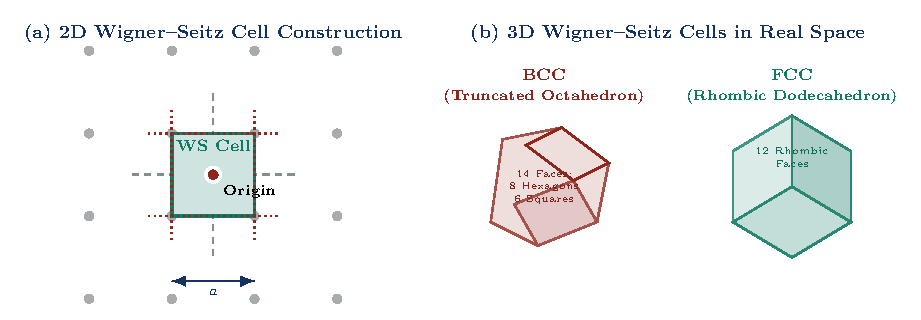
\includegraphics[width=0.95\textwidth]{figures/fig_wigner_seitz.pdf}
\caption{\textbf{Wigner-Seitz Cell Construction.} (Left) 2D direct lattice construction: perpendicular bisectors of vectors to nearest neighbors outline the primitive cell. (Center) 3D Wigner-Seitz cell of a BCC lattice: a truncated octahedron with 8 hexagonal and 6 square faces. (Right) 3D Wigner-Seitz cell of an FCC lattice: a rhombic dodecahedron with 12 identical diamond faces.}
\label{fig:wigner_seitz}
\end{figure}

\textbf{The Wigner-Seitz Primitive Cell:}
The Wigner-Seitz cell is the unique primitive cell that possesses the full point symmetry of the Bravais lattice:
\begin{enumerate}
    \item Select a reference lattice point as the origin.
    \item Draw vectors connecting the origin to all nearest and next-nearest neighbor lattice points.
    \item Construct planes that perpendicularly bisect each of these vectors at their midpoints.
    \item The smallest polyhedron enclosed by these intersecting planes is the \textbf{Wigner-Seitz cell}.
\end{enumerate}

\subsubsection{1.3 The 7 Crystal Systems and 14 Bravais Lattices}
By demanding that translational periodicity is compatible with point-group rotations, exactly \textbf{14 distinct Bravais lattices} arise in three dimensions, grouped into \textbf{7 crystal systems}:

\begin{table}[htbp]
\centering
\small
\begin{tabular}{p{2.6cm}p{3.2cm}p{3.8cm}p{5.2cm}}
\toprule
\textbf{Crystal System} & \textbf{Axial Relations} & \textbf{Interaxial Angles} & \textbf{Bravais Lattices} \\
\midrule
Cubic & $a = b = c$ & $\alpha = \beta = \gamma = 90^\circ$ & Primitive (P), Body-Centered (I), Face-Centered (F) \\
Tetragonal & $a = b \neq c$ & $\alpha = \beta = \gamma = 90^\circ$ & Primitive (P), Body-Centered (I) \\
Orthorhombic & $a \neq b \neq c$ & $\alpha = \beta = \gamma = 90^\circ$ & Primitive (P), Body-Centered (I), Face-Centered (F), Base-Centered (C) \\
Monoclinic & $a \neq b \neq c$ & $\alpha = \gamma = 90^\circ \neq \beta$ & Primitive (P), Base-Centered (C) \\
Triclinic & $a \neq b \neq c$ & $\alpha \neq \beta \neq \gamma \neq 90^\circ$ & Primitive (P) \\
Trigonal (Rhombohedral) & $a = b = c$ & $\alpha = \beta = \gamma < 120^\circ \neq 90^\circ$ & Rhombohedral (R) \\
Hexagonal & $a = b \neq c$ & $\alpha = \beta = 90^\circ, \gamma = 120^\circ$ & Primitive (P) \\
\bottomrule
\end{tabular}
\caption{The 7 crystal systems and 14 Bravais lattices in three dimensions.}
\label{tab:bravais}
\end{table}

\subsubsection{1.4 Common Crystal Structures (SC, BCC, FCC, Diamond, HCP)}

\begin{figure}[htbp]
\centering
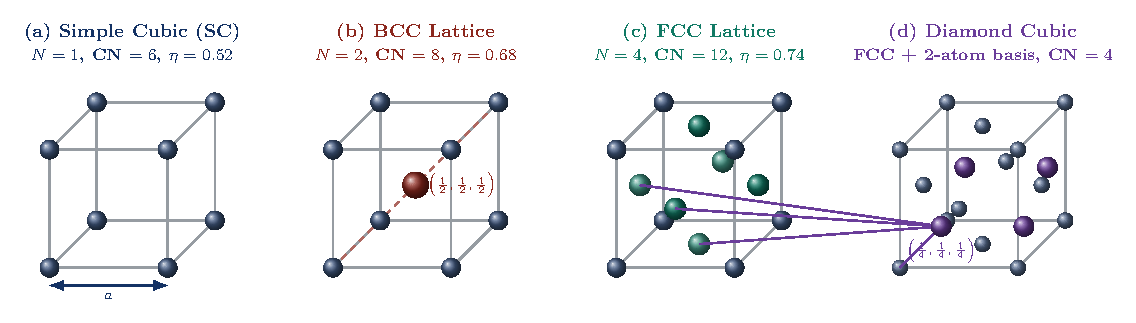
\includegraphics[width=0.98\textwidth]{figures/fig_crystal_unit_cells.pdf}
\caption{\textbf{Fundamental Cubic Crystal Structures.} (a) Simple Cubic (SC) with coordination number $Z=6$. (b) Body-Centered Cubic (BCC) with body-centered atom at $(1/2,1/2,1/2)$ and $Z=8$. (c) Face-Centered Cubic (FCC) with atoms at face centers and $Z=12$. (d) Diamond Cubic structure formed by an FCC lattice with a two-atom basis at $(0,0,0)$ and $(1/4,1/4,1/4)$, yielding tetrahedral coordination $Z=4$.}
\label{fig:crystal_cells}
\end{figure}

\begin{itemize}[leftmargin=1.5em]
    \item \textbf{Simple Cubic (SC):} 1 atom per cell ($8 \times \frac{1}{8}$). Atoms touch along cube edge: $a = 2r$. Coordination $Z = 6$. Atomic packing factor (APF) = $\frac{\pi}{6} \approx 0.524$.
    \item \textbf{Body-Centered Cubic (BCC):} 2 atoms per cell ($8 \times \frac{1}{8} + 1$). Atoms touch along body diagonal: $4r = a\sqrt{3}$. Coordination $Z = 8$. APF = $\frac{\pi\sqrt{3}}{8} \approx 0.680$.
    \item \textbf{Face-Centered Cubic (FCC):} 4 atoms per cell ($8 \times \frac{1}{8} + 6 \times \frac{1}{2}$). Atoms touch along face diagonal: $4r = a\sqrt{2}$. Coordination $Z = 12$. APF = $\frac{\pi}{3\sqrt{2}} \approx 0.7405$.
    \item \textbf{Hexagonal Close-Packed (HCP):} ABABAB\ldots{} stacking. Primitive cell contains 2 atoms. Ideal axial ratio $c/a = \sqrt{8/3} \approx 1.633$. Coordination $Z = 12$, APF $\approx 0.7405$.
\end{itemize}

\begin{solbox}[Worked Example: Derivation of the FCC Packing Fraction (Problem 1.1)]
\textbf{Problem Statement:} Show that the maximum packing fraction of hard spheres in an FCC crystal is $0.74$.

\textbf{Detailed Derivation:}
\begin{enumerate}
    \item In an FCC lattice, spheres touch along the face diagonal of the conventional cubic cell. The length of the face diagonal is $a\sqrt{2}$.
    \item Along this diagonal, there is one corner radius, one full sphere diameter, and another corner radius:
    \begin{equation}
    4r = a\sqrt{2} \implies r = \frac{a\sqrt{2}}{4}
    \end{equation}
    \item The number of effective spheres in the conventional FCC cell is:
    \begin{equation}
    N_{\text{eff}} = 8 \times \frac{1}{8} \text{ (corners)} + 6 \times \frac{1}{2} \text{ (faces)} = 1 + 3 = 4
    \end{equation}
    \item The total volume occupied by the 4 spherical atoms is:
    \begin{equation}
    V_{\text{atoms}} = 4 \times \left(\frac{4}{3}\pi r^3\right) = \frac{16\pi}{3} r^3 = \frac{16\pi}{3}\left(\frac{a\sqrt{2}}{4}\right)^3 = \frac{16\pi}{3} \frac{2\sqrt{2}a^3}{64} = \frac{\pi\sqrt{2}}{6} a^3
    \end{equation}
    \item The packing fraction $\eta$ is the ratio of atomic volume to total cell volume $V_{\text{cell}} = a^3$:
    \begin{equation}
    \eta = \frac{V_{\text{atoms}}}{V_{\text{cell}}} = \frac{\pi\sqrt{2}}{6} = \frac{\pi}{3\sqrt{2}} \approx \mathbf{0.7405 \quad (74.05\%)}
    \end{equation}
\end{enumerate}
\end{solbox}

\begin{solbox}[Worked Example: Atom Count in the Diamond Structure (Problem 1.2)]
\textbf{Problem Statement:} Determine the number of atoms in the conventional unit cell of the diamond crystal structure.

\textbf{Solution:}
\begin{enumerate}
    \item The diamond structure consists of a Face-Centered Cubic (FCC) Bravais lattice with a \textbf{two-atom basis}:
    \begin{equation}
    \mathbf{r}_1 = (0,0,0), \qquad \mathbf{r}_2 = \left(\frac{1}{4}, \frac{1}{4}, \frac{1}{4}\right)
    \end{equation}
    \item An FCC conventional cell possesses $N_{\text{lattice}} = 4$ lattice points.
    \item Since each lattice point is decorated by 2 identical carbon atoms, the total number of atoms per conventional cell is:
    \begin{equation}
    N_{\text{total}} = 4 \times 2 = \mathbf{8 \text{ atoms}}
    \end{equation}
    \item Geometrically, 4 atoms occupy the standard FCC sites (corners and face centers) and 4 atoms occupy tetrahedral interstitial sites located entirely within the cubic cell.
\end{enumerate}
\end{solbox}

\subsection{PART B: Miller Indices, Planes, and Directions}

\subsubsection{1.5 Crystal Directions \texorpdfstring{$[uvw]$}{[uvw]} and Families \texorpdfstring{$\langle uvw \rangle$}{<uvw>}}
A crystal direction is the vector connecting two lattice points:
\begin{equation}
\mathbf{T} = u\mathbf{a}_1 + v\mathbf{a}_2 + w\mathbf{a}_3
\end{equation}
where $u, v, w$ are the smallest integers having the same ratio. Square brackets $[uvw]$ denote an individual direction, and angle brackets $\langle uvw \rangle$ denote the set of all symmetry-equivalent directions (e.g., $\langle 100 \rangle$ represents $[100], [\bar{1}00], [010], [0\bar{1}0], [001], [00\bar{1}]$ in a cubic crystal).

\subsubsection{1.6 Miller Indices \texorpdfstring{$(hkl)$}{(hkl)} for Lattice Planes}

\begin{figure}[htbp]
\centering
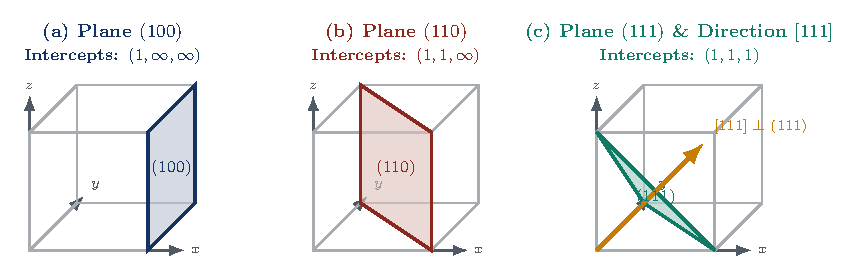
\includegraphics[width=0.96\textwidth]{figures/fig_miller_planes.pdf}
\caption{\textbf{Miller Planes in a Cubic Unit Cell.} (Left) $(100)$ plane intercepting $x=a$ and parallel to $y, z$. (Center) $(110)$ plane cutting diagonal face with normal along $[110]$. (Right) $(111)$ plane forming an equilateral triangle with intercepts at $x=a, y=a, z=a$, explicitly displaying the surface normal direction $[111]$.}
\label{fig:miller_planes}
\end{figure}

Miller indices $(hkl)$ uniquely define a parallel stack of equidistant lattice planes:
\begin{enumerate}
    \item Determine intercepts of the plane along the three crystallographic axes in units of $a, b, c$: $(x_1, x_2, x_3)$. If a plane is parallel to an axis, its intercept is $\infty$.
    \item Take the reciprocals: $(1/x_1, 1/x_2, 1/x_3)$.
    \item Clear fractions to obtain the smallest coprimary integers: $(hkl)$.
    \item A bar over an index indicates an intercept on the negative coordinate axis: $(h\bar{k}l)$.
    \item Curly braces $\{hkl\}$ denote the family of symmetry-equivalent planes.
\end{enumerate}

\begin{solbox}[Worked Example: Determining Miller Indices from Intercepts (Problem 1.4)]
\textbf{Problem Statement:} A crystal plane intercepts the axes at $2a$, $3b$, and $6c$. Determine its Miller indices.

\textbf{Solution:}
\begin{enumerate}
    \item Fractional intercepts: $(2, 3, 6)$.
    \item Reciprocals: $\left(\frac{1}{2}, \frac{1}{3}, \frac{1}{6}\right)$.
    \item Multiply by the lowest common multiple ($\text{LCM} = 6$):
    \begin{equation}
    6 \times \left(\frac{1}{2}, \frac{1}{3}, \frac{1}{6}\right) = (3, 2, 1)
    \end{equation}
    \item The Miller indices of the plane are $\mathbf{(321)}$.
\end{enumerate}
\end{solbox}

\subsubsection{1.7 Interplanar Spacing Formulas}
The perpendicular distance $d_{hkl}$ between adjacent parallel lattice planes of the family $(hkl)$ is:
\begin{itemize}[leftmargin=1.5em]
    \item \textbf{Cubic System ($a=b=c$):}
    \begin{equation}
    d_{hkl} = \frac{a}{\sqrt{h^2 + k^2 + l^2}}
    \end{equation}
    \item \textbf{Tetragonal System ($a=b\neq c$):}
    \begin{equation}
    \frac{1}{d_{hkl}^2} = \frac{h^2 + k^2}{a^2} + \frac{l^2}{c^2}
    \end{equation}
    \item \textbf{Orthorhombic System ($a\neq b\neq c$):}
    \begin{equation}
    \frac{1}{d_{hkl}^2} = \frac{h^2}{a^2} + \frac{k^2}{b^2} + \frac{l^2}{c^2}
    \end{equation}
\end{itemize}

\begin{solbox}[Worked Example: Physical Density and Interplanar Spacing in Copper (Problems 1.5 \& 4.19)]
\textbf{Problem Statement:} Metallic copper crystallizes in FCC with lattice constant $a = 3.61\,\text{\AA}$ and molar mass $M = 63.55\,\text{g/mol}$.
\begin{enumerate}[label=(\alph*)]
    \item Calculate the metallic atomic radius $r_{\text{Cu}}$.
    \item Calculate the theoretical density $\rho_{\text{Cu}}$.
    \item Calculate the interplanar spacings $d_{220}$ and $d_{111}$.
\end{enumerate}

\textbf{Solution:}
\begin{enumerate}[label=(\alph*)]
    \item In FCC, atoms touch along face diagonals:
    \begin{equation}
    r = \frac{a\sqrt{2}}{4} = \frac{3.61 \times 1.4142}{4} = \mathbf{1.276\,\text{\AA}} = 0.1276\,\text{nm}
    \end{equation}
    \item The mass density of a conventional unit cell containing $Z = 4$ copper atoms is:
    \begin{equation}
    \rho = \frac{Z \cdot M}{N_A \cdot a^3} = \frac{4 \times (63.55 \times 10^{-3}\,\text{kg/mol})}{(6.022 \times 10^{23}\,\text{mol}^{-1}) \times (3.61 \times 10^{-10}\,\text{m})^3} = \mathbf{8933\,\text{kg/m}^3} = \mathbf{8.93\,\text{g/cm}^3}
    \end{equation}
    \item Interplanar spacings:
    \begin{align}
    d_{220} &= \frac{a}{\sqrt{2^2 + 2^2 + 0^2}} = \frac{3.61\,\text{\AA}}{\sqrt{8}} = \frac{3.61}{2.8284} = \mathbf{1.276\,\text{\AA}} \\
    d_{111} &= \frac{a}{\sqrt{1^2 + 1^2 + 1^2}} = \frac{3.61\,\text{\AA}}{\sqrt{3}} = \frac{3.61}{1.7321} = \mathbf{2.084\,\text{\AA}}
    \end{align}
\end{enumerate}
\end{solbox}

\subsubsection{1.8 Important Prototype Crystal Structures}
\begin{itemize}[leftmargin=1.5em]
    \item \textbf{NaCl (Rock Salt):} FCC Bravais lattice with a two-ion basis: $\text{Na}^+$ at $(0,0,0)$ and $\text{Cl}^-$ at $(1/2,0,0)$. Each ion is coordinated by 6 octahedrally arranged nearest neighbors of opposite charge ($Z=6$). Contains 4 NaCl formula units per cell.
    \item \textbf{CsCl (Cesium Chloride):} Simple Cubic Bravais lattice with $\text{Cs}^+$ at $(0,0,0)$ and $\text{Cl}^-$ at $(1/2,1/2,1/2)$. 8-fold cubic coordination ($Z=8$). Contains 1 CsCl formula unit per cell.
    \item \textbf{Diamond Structure:} FCC lattice with basis $(0,0,0)$ and $(1/4,1/4,1/4)$. Every atom is $sp^3$-hybridized and tetrahedrally coordinated ($Z=4$).
    \item \textbf{Zinc Blende (Sphalerite, ZnS):} Same geometric framework as diamond, but Zn atoms reside at FCC sites and S atoms reside at the $(1/4,1/4,1/4)$ tetrahedral sites. Lacks inversion symmetry.
\end{itemize}

\newpage

% ==================== LECTURE 2 ====================
\section{Lecture 2: Reciprocal Lattice \& Diffraction Conditions}

\subsection{PART A: Reciprocal Lattice Definition and Geometric Duality}

\subsubsection{2.1 Physical Motivation}
Why do physicists describe crystals in reciprocal space?
\begin{itemize}[leftmargin=1.5em]
    \item In diffraction, incident radiation (X-rays, neutrons, electrons) possesses a wave vector $\mathbf{k}$ with $|\mathbf{k}| = 2\pi/\lambda$. Interference conditions naturally live in Fourier wave-vector space.
    \item Any physical property sharing direct-space lattice periodicity (electron density $n(\mathbf{r})$, crystal potential $U(\mathbf{r})$) expands as a discrete Fourier series over reciprocal lattice vectors $\mathbf{G}$.
    \item Electron energy bands $E_n(\mathbf{k})$ and phonon dispersions $\omega_s(\mathbf{q})$ are uniquely defined in the first Brillouin zone.
\end{itemize}

\subsubsection{2.2 Mathematical Formulation of the Reciprocal Lattice}
Given primitive translation vectors $\mathbf{a}_1, \mathbf{a}_2, \mathbf{a}_3$ of a direct lattice, the primitive vectors of the reciprocal lattice $\mathbf{b}_1, \mathbf{b}_2, \mathbf{b}_3$ are defined by the fundamental orthogonality relation:
\begin{equation}
\mathbf{a}_i \cdot \mathbf{b}_j = 2\pi \delta_{ij} = \begin{cases} 2\pi & i = j \\ 0 & i \neq j \end{cases}
\end{equation}

Explicitly, in terms of direct vectors and primitive volume $V = \mathbf{a}_1 \cdot (\mathbf{a}_2 \times \mathbf{a}_3)$:
\begin{equation}
\mathbf{b}_1 = 2\pi \frac{\mathbf{a}_2 \times \mathbf{a}_3}{\mathbf{a}_1 \cdot (\mathbf{a}_2 \times \mathbf{a}_3)}, \qquad
\mathbf{b}_2 = 2\pi \frac{\mathbf{a}_3 \times \mathbf{a}_1}{\mathbf{a}_1 \cdot (\mathbf{a}_2 \times \mathbf{a}_3)}, \qquad
\mathbf{b}_3 = 2\pi \frac{\mathbf{a}_1 \times \mathbf{a}_2}{\mathbf{a}_1 \cdot (\mathbf{a}_2 \times \mathbf{a}_3)}
\end{equation}
Any reciprocal lattice vector is a linear integer combination:
\begin{equation}
\mathbf{G} = h\mathbf{b}_1 + k\mathbf{b}_2 + l\mathbf{b}_3, \qquad h, k, l \in \mathbb{Z}
\end{equation}

\begin{solbox}[Worked Example: Proof that the Reciprocal of BCC is FCC (Problem 2.8)]
\textbf{Problem Statement:} Derive the primitive reciprocal lattice vectors for a direct BCC lattice of lattice constant $a$, and prove that the reciprocal lattice is Face-Centered Cubic (FCC).

\textbf{Mathematical Derivation:}
\begin{enumerate}
    \item Symmetric primitive translation vectors of the BCC direct lattice:
    \begin{equation}
    \mathbf{a}_1 = \frac{a}{2}(-\hat{x} + \hat{y} + \hat{z}), \quad
    \mathbf{a}_2 = \frac{a}{2}(\hat{x} - \hat{y} + \hat{z}), \quad
    \mathbf{a}_3 = \frac{a}{2}(\hat{x} + \hat{y} - \hat{z})
    \end{equation}
    \item Compute the cross product $\mathbf{a}_2 \times \mathbf{a}_3$:
    \begin{align}
    \mathbf{a}_2 \times \mathbf{a}_3 &= \frac{a^2}{4} \begin{vmatrix} \hat{x} & \hat{y} & \hat{z} \\ 1 & -1 & 1 \\ 1 & 1 & -1 \end{vmatrix} \notag\\
    &= \frac{a^2}{4} \left[ \hat{x}(1-1) - \hat{y}(-1-1) + \hat{z}(1 - (-1)) \right] \notag\\
    &= \frac{a^2}{4} (2\hat{y} + 2\hat{z}) = \frac{a^2}{2}(\hat{y} + \hat{z})
    \end{align}
    \item Compute the primitive direct volume $V$:
    \begin{equation}
    V = \mathbf{a}_1 \cdot (\mathbf{a}_2 \times \mathbf{a}_3) = \frac{a}{2}(-\hat{x} + \hat{y} + \hat{z}) \cdot \frac{a^2}{2}(\hat{y} + \hat{z}) = \frac{a^3}{4}(1 + 1) = \frac{a^3}{2}
    \end{equation}
    \item The first reciprocal primitive vector is:
    \begin{equation}
    \mathbf{b}_1 = 2\pi \frac{\mathbf{a}_2 \times \mathbf{a}_3}{V} = 2\pi \frac{\frac{a^2}{2}(\hat{y} + \hat{z})}{\frac{a^3}{2}} = \frac{2\pi}{a}(\hat{y} + \hat{z})
    \end{equation}
    \item By cyclic permutation of axes:
    \begin{equation}
    \mathbf{b}_2 = \frac{2\pi}{a}(\hat{x} + \hat{z}), \qquad \mathbf{b}_3 = \frac{2\pi}{a}(\hat{x} + \hat{y})
    \end{equation}
    \item Notice that these vectors have exactly the form of primitive vectors of a \textbf{Face-Centered Cubic (FCC)} direct lattice:
    \begin{equation}
    \mathbf{b}_1 = \frac{A}{2}(\hat{y} + \hat{z}), \quad \mathbf{b}_2 = \frac{A}{2}(\hat{x} + \hat{z}), \quad \mathbf{b}_3 = \frac{A}{2}(\hat{x} + \hat{y}) \quad \text{with } A = \frac{4\pi}{a}
    \end{equation}
    Hence, the reciprocal lattice of a BCC lattice of parameter $a$ is an \textbf{FCC lattice} with conventional cubic edge $4\pi/a$. $\quad\blacksquare$
\end{enumerate}
\end{solbox}

\subsubsection{2.3 Geometric Proof: \texorpdfstring{$\mathbf{G}_{hkl}$}{G\_hkl} is Normal to the \texorpdfstring{$(hkl)$}{(hkl)} Planes}

\begin{solbox}[Worked Example: Proof of Reciprocal Normal Property (Problem 2.9)]
\textbf{Problem Statement:} Prove that $\mathbf{G}_{hkl} = h\mathbf{b}_1 + k\mathbf{b}_2 + l\mathbf{b}_3$ is perpendicular to the crystal plane $(hkl)$.

\textbf{Proof:}
\begin{enumerate}
    \item By definition of Miller indices, the plane $(hkl)$ nearest to the origin intersects the crystallographic axes at the points:
    \begin{equation}
    \mathbf{P}_1 = \frac{\mathbf{a}_1}{h}, \qquad \mathbf{P}_2 = \frac{\mathbf{a}_2}{k}, \qquad \mathbf{P}_3 = \frac{\mathbf{a}_3}{l}
    \end{equation}
    \item Form two independent vectors lying wholly within this $(hkl)$ plane:
    \begin{equation}
    \mathbf{u} = \mathbf{P}_1 - \mathbf{P}_2 = \frac{\mathbf{a}_1}{h} - \frac{\mathbf{a}_2}{k}, \qquad \mathbf{v} = \mathbf{P}_2 - \mathbf{P}_3 = \frac{\mathbf{a}_2}{k} - \frac{\mathbf{a}_3}{l}
    \end{equation}
    \item Take the scalar product of $\mathbf{G}_{hkl}$ with $\mathbf{u}$, applying $\mathbf{a}_i \cdot \mathbf{b}_j = 2\pi\delta_{ij}$:
    \begin{align}
    \mathbf{G}_{hkl} \cdot \mathbf{u} &= (h\mathbf{b}_1 + k\mathbf{b}_2 + l\mathbf{b}_3) \cdot \left(\frac{\mathbf{a}_1}{h} - \frac{\mathbf{a}_2}{k}\right) \notag\\
    &= \frac{h}{h}(\mathbf{b}_1 \cdot \mathbf{a}_1) - \frac{h}{k}(\mathbf{b}_1 \cdot \mathbf{a}_2) + \frac{k}{h}(\mathbf{b}_2 \cdot \mathbf{a}_1) - \frac{k}{k}(\mathbf{b}_2 \cdot \mathbf{a}_2) + \dots \notag\\
    &= 1 \times (2\pi) - 0 + 0 - 1 \times (2\pi) = 2\pi - 2\pi = \mathbf{0}
    \end{align}
    \item Similarly, evaluating $\mathbf{G}_{hkl} \cdot \mathbf{v}$:
    \begin{equation}
    \mathbf{G}_{hkl} \cdot \left(\frac{\mathbf{a}_2}{k} - \frac{\mathbf{a}_3}{l}\right) = 2\pi - 2\pi = \mathbf{0}
    \end{equation}
    \item Because $\mathbf{G}_{hkl}$ is orthogonal to two linearly independent vectors spanning the plane, it is strictly perpendicular to the entire plane family:
    \begin{equation}
    \mathbf{G}_{hkl} \perp (hkl)
    \end{equation}
    \item The interplanar spacing $d_{hkl}$ is the projection of $\mathbf{P}_1$ along the unit normal $\hat{\mathbf{n}} = \mathbf{G}_{hkl}/|\mathbf{G}_{hkl}|$:
    \begin{equation}
    d_{hkl} = \mathbf{P}_1 \cdot \frac{\mathbf{G}_{hkl}}{|\mathbf{G}_{hkl}|} = \frac{\mathbf{a}_1}{h} \cdot \frac{h\mathbf{b}_1 + k\mathbf{b}_2 + l\mathbf{b}_3}{|\mathbf{G}_{hkl}|} = \frac{\mathbf{a}_1 \cdot \mathbf{b}_1}{|\mathbf{G}_{hkl}|} = \mathbf{\frac{2\pi}{|\mathbf{G}_{hkl}|}} \quad\blacksquare
    \end{equation}
\end{enumerate}
\end{solbox}

\subsubsection{2.4 Brillouin Zones: Wigner-Seitz Cells of the Reciprocal Lattice}
The \textbf{First Brillouin Zone (1st BZ)} is defined as the Wigner-Seitz primitive cell of the reciprocal lattice. It contains all wave vectors $\mathbf{k}$ that can reach no reciprocal lattice point without crossing a Bragg reflection plane.

\begin{figure}[htbp]
\centering
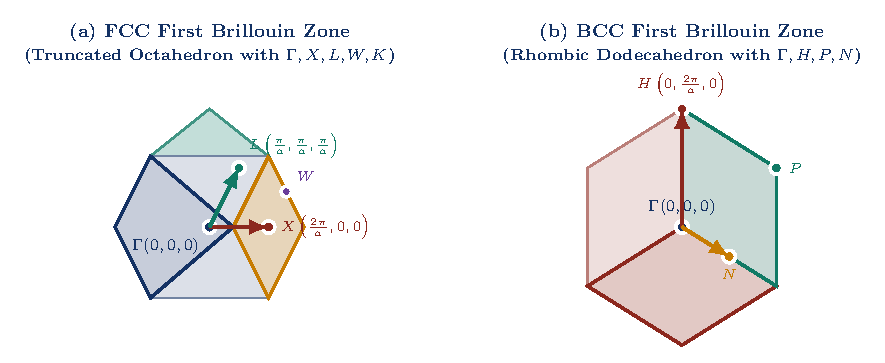
\includegraphics[width=0.96\textwidth]{figures/fig_brillouin_zones.pdf}
\caption{\textbf{First Brillouin Zones of Cubic Lattices.} (Left) 1st BZ of an FCC direct lattice (reciprocal is BCC): a truncated octahedron showing high-symmetry points $\Gamma(0,0,0)$, $X$, $L$, $W$, and $K$. (Right) 1st BZ of a BCC direct lattice (reciprocal is FCC): a rhombic dodecahedron with 12 diamond faces and high-symmetry points $\Gamma(0,0,0)$, $H$, $P$, and $N$.}
\label{fig:brillouin_zones}
\end{figure}

\subsection{PART B: Bragg's Law, Laue Condition, and Ewald Sphere}

\subsubsection{2.5 Bragg's Law vs. von Laue Condition}

\begin{figure}[htbp]
\centering
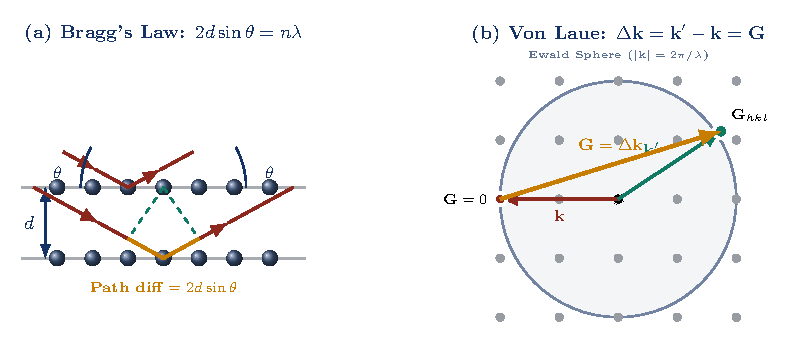
\includegraphics[width=0.96\textwidth]{figures/fig_bragg_diffraction.pdf}
\caption{\textbf{Diffraction Geometry in Real and Reciprocal Space.} (Left) Bragg's Law in real space: specular reflection from lattice planes separated by distance $d_{hkl}$, generating geometric path difference $2d\sin\theta = n\lambda$. (Right) The Ewald Sphere construction in reciprocal space: incident wave vector $\mathbf{k}$ terminates at reciprocal origin $O$. A sphere of radius $k = 2\pi/\lambda$ centered at $C$ intersects reciprocal lattice point $P$, satisfying the von Laue vector condition $\Delta\mathbf{k} = \mathbf{k}' - \mathbf{k} = \mathbf{G}$.}
\label{fig:bragg_diffraction}
\end{figure}

\begin{keybox}[Equivalence of Bragg's Law and Laue Condition]
\begin{enumerate}
    \item \textbf{Bragg's Law (Real Space):}
    \begin{equation}
    2d_{hkl}\sin\theta = n\lambda
    \end{equation}
    \item \textbf{Laue Condition (Reciprocal Space):}
    \begin{equation}
    \Delta\mathbf{k} = \mathbf{k}' - \mathbf{k} = \mathbf{G}
    \end{equation}
    For elastic scattering, $|\mathbf{k}'| = |\mathbf{k}| = 2\pi/\lambda$. Squaring both sides:
    \begin{equation}
    |\mathbf{k}'|^2 = |\mathbf{k} + \mathbf{G}|^2 \implies k^2 = k^2 + 2\mathbf{k}\cdot\mathbf{G} + G^2 \implies 2\mathbf{k}\cdot\mathbf{G} + G^2 = 0
    \end{equation}
    Since $\mathbf{k}$ makes an angle $(\frac{\pi}{2} + \theta)$ with $\mathbf{G}$:
    \begin{equation}
    2\left(\frac{2\pi}{\lambda}\right) G \sin\theta = G^2 \implies 2\sin\theta = \frac{G}{2\pi/\lambda} = \frac{2\pi/d_{hkl}}{2\pi/\lambda} \lambda = \frac{\lambda}{d_{hkl}} \implies \mathbf{2d_{hkl}\sin\theta = \lambda}
    \end{equation}
\end{enumerate}
\end{keybox}

\begin{solbox}[Worked Example: Bragg Angle in Rock Salt NaCl (Problem 2.10)]
\textbf{Problem Statement:} Calculate the glancing angle $\theta$ and detector angle $2\theta$ for the $(200)$ reflection in NaCl ($a = 5.64\,\text{\AA}$) using Cu K$\alpha$ radiation ($\lambda = 1.54\,\text{\AA}$).

\textbf{Solution:}
\begin{enumerate}
    \item Interplanar spacing for $(200)$ in cubic NaCl:
    \begin{equation}
    d_{200} = \frac{a}{\sqrt{2^2 + 0^2 + 0^2}} = \frac{5.64\,\text{\AA}}{2} = 2.82\,\text{\AA}
    \end{equation}
    \item By Bragg's law ($n=1$):
    \begin{equation}
    \sin\theta = \frac{\lambda}{2d_{200}} = \frac{1.54\,\text{\AA}}{2 \times 2.82\,\text{\AA}} = \frac{1.54}{5.64} = 0.27305
    \end{equation}
    \item Calculating the angles:
    \begin{align}
    \theta &= \arcsin(0.27305) = \mathbf{15.85^\circ} \\
    2\theta &= 2 \times 15.85^\circ = \mathbf{31.70^\circ}
    \end{align}
\end{enumerate}
\end{solbox}

\subsubsection{2.6 The Geometric Structure Factor and Systematic Absences}
When a unit cell contains multiple atoms at fractional coordinates $\mathbf{r}_j = x_j\mathbf{a}_1 + y_j\mathbf{a}_2 + z_j\mathbf{a}_3$, the total scattered amplitude is the superposition of waves scattered by each individual atomic electron cloud:
\begin{equation}
F_{hkl} = \sum_{j=1}^{N_{\text{basis}}} f_j \exp\left[i\mathbf{G}_{hkl}\cdot\mathbf{r}_j\right] = \sum_{j=1}^{N_{\text{basis}}} f_j \exp\left[2\pi i(hx_j + ky_j + lz_j)\right]
\end{equation}
The observed Bragg peak intensity is proportional to $|F_{hkl}|^2$:
\begin{equation}
I_{hkl} \propto |F_{hkl}|^2
\end{equation}
If $F_{hkl} = 0$, destructive interference completely suppresses the diffracted beam, yielding a \textbf{systematic absence (extinction)}.

\begin{figure}[htbp]
\centering
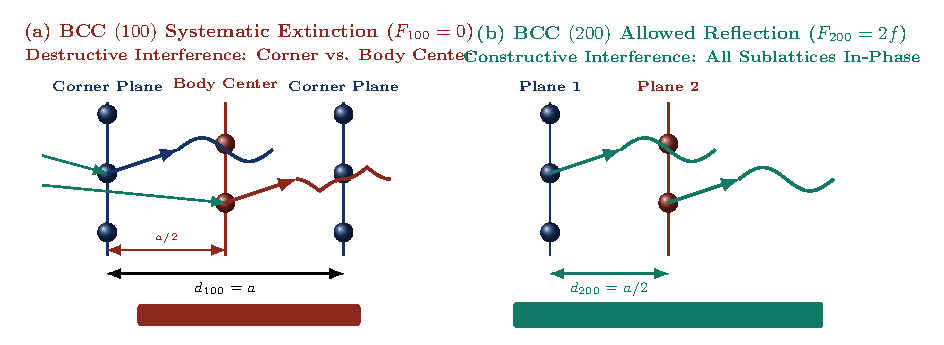
\includegraphics[width=0.96\textwidth]{figures/fig_structure_factor.pdf}
\caption{\textbf{Origin of Systematic Absences in BCC Lattices.} (Left) Destructive interference for the $(100)$ plane: the body-centered plane midway at $x = a/2$ scatters exactly $\pi$ out of phase ($\Delta\phi = \pi$), resulting in complete wave cancellation ($F_{100} = 0$). (Right) Constructive interference for the $(200)$ plane: the path difference is a full wavelength $\lambda$, waves add in phase ($\Delta\phi = 2\pi$), giving a bright diffraction peak ($F_{200} = 2f$).}
\label{fig:structure_factor}
\end{figure}

\begin{solbox}[Worked Example: Extinction in BCC vs. Simple Cubic (Problem 2.12)]
\textbf{Problem Statement:} Explain why the $(100)$ reflection is forbidden in BCC but allowed in Simple Cubic.

\textbf{Derivation:}
\begin{enumerate}
    \item A conventional BCC cell contains two identical atoms: at $(0,0,0)$ and $\left(\frac{1}{2}, \frac{1}{2}, \frac{1}{2}\right)$.
    \item The structure factor is:
    \begin{equation}
    F_{hkl} = f \left[ e^{2\pi i(0)} + e^{2\pi i(\frac{h}{2} + \frac{k}{2} + \frac{l}{2})} \right] = f \left[ 1 + e^{i\pi(h+k+l)} \right]
    \end{equation}
    \item Because $e^{i\pi m} = (-1)^m$:
    \begin{equation}
    F_{hkl} = \begin{cases} 2f & \text{if } h+k+l \text{ is even} \\ 0 & \text{if } h+k+l \text{ is odd} \end{cases}
    \end{equation}
    \item For the $(100)$ plane: $h+k+l = 1 + 0 + 0 = 1$ (odd). Thus:
    \begin{equation}
    F_{100} = f[1 + (-1)^1] = \mathbf{0} \quad \implies \text{Systematic absence!}
    \end{equation}
    \item In Simple Cubic (1 atom at $(0,0,0)$), there is no interleaving body-centered atom: $F_{100} = f \neq 0$, so $(100)$ produces a bright reflection.
\end{enumerate}
\end{solbox}

\newpage

% ==================== LECTURE 3 ====================
\section{Lecture 3: Experimental Diffraction Methods \& Crystal Symmetry}

\subsection{PART A: Experimental X-ray Diffraction Techniques}

\subsubsection{3.1 Three Standard Experimental Methods}
To observe diffraction, the Ewald sphere of radius $k = 2\pi/\lambda$ must intersect a reciprocal lattice point $\mathbf{G}_{hkl}$. Since three conditions must be satisfied ($2d\sin\theta = \lambda$), one must provide an experimental degree of freedom:

\begin{table}[htbp]
\centering
\small
\begin{tabular}{lllp{6cm}}
\toprule
\textbf{Method} & \textbf{Wavelength $\lambda$} & \textbf{Crystal Specimen} & \textbf{Primary Scientific Application} \\
\midrule
\textbf{Laue Method} & Continuous (White) & Stationary Single Crystal & Rapid orientation of single crystals; determination of point-group crystal symmetry. \\
\textbf{Rotating Crystal} & Monochromatic & Rotating Single Crystal & Determination of unknown unit cell dimensions from layer-line spacing. \\
\textbf{Powder Method} & Monochromatic & Polycrystalline Powder & Identification of unknown phases; precise lattice parameter determination; structure solution. \\
\bottomrule
\end{tabular}
\caption{Comparison of fundamental experimental X-ray diffraction methods.}
\label{tab:xrd_methods}
\end{table}

\subsubsection{3.2 Debye-Scherrer Powder Method and Cubic Indexing}
In a fine polycrystalline powder, millions of microscopic crystal grains are randomly oriented. For any allowed $(hkl)$ plane, there are always crystallites oriented at the precise Bragg angle $\theta$. The diffracted rays form a continuous coaxial cone of semi-angle $2\theta$ around the incident beam (the \textbf{Debye-Scherrer cone}).

For any cubic crystal, the diffraction equation is:
\begin{equation}
\sin^2\theta = \frac{\lambda^2}{4a^2}(h^2 + k^2 + l^2) = \frac{\lambda^2}{4a^2} N, \qquad \text{where } N \equiv h^2 + k^2 + l^2
\end{equation}
Because $\frac{\lambda^2}{4a^2}$ is a constant for a given experiment, the values of $\sin^2\theta$ for consecutive peaks are proportional to integers $N$:

\begin{keybox}[Characteristic Cubic Extinction Sequences]
\begin{itemize}[leftmargin=1.5em]
    \item \textbf{Simple Cubic (SC):} All integer $N$ allowed: $N = 1, 2, 3, 4, 5, 6, 8, \dots$ (Notice $N=7$ is mathematically impossible since no three squares sum to 7).
    \item \textbf{Body-Centered Cubic (BCC):} $h+k+l = \text{even} \implies N = 2, 4, 6, 8, 10, 12, 14, 16, \dots$
    \item \textbf{Face-Centered Cubic (FCC):} $h,k,l$ all odd or all even $\implies N = 3, 4, 8, 11, 12, 16, 19, 20, \dots$
    \item \textbf{Diamond Cubic:} FCC-allowed with $h+k+l \neq 4n+2 \implies N = 3, 8, 11, 16, 19, 24, 27, \dots$
\end{itemize}
\end{keybox}

\begin{solbox}[Worked Example: Indexing the Powder Pattern of BCC Iron (Problem 3.13)]
\textbf{Problem Statement:} Index the first five diffraction lines of BCC $\alpha$-iron ($a = 2.87\,\text{\AA}$) using $\text{Cu K}\alpha$ radiation ($\lambda = 1.54\,\text{\AA}$). Calculate their respective $2\theta$ angles.

\textbf{Solution:}
\begin{enumerate}
    \item The prefactor is:
    \begin{equation}
    A = \frac{\lambda}{2a} = \frac{1.54\,\text{\AA}}{2 \times 2.87\,\text{\AA}} = 0.26829 \implies A^2 = 0.07198
    \end{equation}
    \item In BCC, the allowed $N = h^2 + k^2 + l^2$ values are even integers: $2, 4, 6, 8, 10$.
    \item Tabulate the reflections:
    \begin{center}
    \begin{tabular}{ccccc}
    \toprule
    $\mathbf{(hkl)}$ & $\mathbf{N}$ & $\mathbf{\sin\theta = A\sqrt{N}}$ & $\mathbf{\theta}$ & $\mathbf{2\theta}$ \\
    \midrule
    $(110)$ & 2 & $0.26829 \times 1.4142 = 0.3794$ & $22.30^\circ$ & $\mathbf{44.60^\circ}$ \\
    $(200)$ & 4 & $0.26829 \times 2.0000 = 0.5366$ & $32.45^\circ$ & $\mathbf{64.90^\circ}$ \\
    $(211)$ & 6 & $0.26829 \times 2.4495 = 0.6572$ & $41.08^\circ$ & $\mathbf{82.16^\circ}$ \\
    $(220)$ & 8 & $0.26829 \times 2.8284 = 0.7589$ & $49.37^\circ$ & $\mathbf{98.74^\circ}$ \\
    $(310)$ & 10 & $0.26829 \times 3.1623 = 0.8484$ & $58.04^\circ$ & $\mathbf{116.08^\circ}$ \\
    \bottomrule
    \end{tabular}
    \end{center}
\end{enumerate}
\end{solbox}

\subsubsection{3.3 Multiplicity Factor \texorpdfstring{$p_{hkl}$}{p\_hkl}}
In a powder pattern, all symmetry-equivalent planes with the exact same spacing $d_{hkl}$ scatter at identical $2\theta$ angles and contribute constructively to the same powder line. The number of such equivalent planes is the \textbf{multiplicity factor} $p$.

\begin{solbox}[Worked Example: Multiplicity of $\{110\}$ in Cubic Crystals (Problem 3.15)]
\textbf{Problem Statement:} Calculate the multiplicity factor for $\{110\}$ planes in a cubic crystal.

\textbf{Solution:}
In a cubic crystal with full octahedral symmetry:
\begin{enumerate}
    \item Permutations of the zero index across the 3 coordinates: 3 choices ($xy$, $yz$, $zx$).
    \item Sign combinations of the two non-zero indices: $(\pm 1, \pm 1)$, giving $2 \times 2 = 4$ combinations.
    \item Total number of distinct planes in the family:
    \begin{equation}
    p = 3 \times 4 = \mathbf{12}
    \end{equation}
    Explicit list: $(110), (1\bar{1}0), (\bar{1}10), (\bar{1}\bar{1}0), (101), (10\bar{1}), (\bar{1}01), (\bar{1}0\bar{1}), (011), (01\bar{1}), (0\bar{1}1), (0\bar{1}\bar{1})$.
\end{enumerate}
\end{solbox}

\subsection{PART B: Crystal Symmetry, Point Groups, and Neumann's Principle}

\subsubsection{3.4 The Crystallographic Restriction Theorem}

\begin{solbox}[Worked Example: Incompatibility of 5-Fold Symmetry (Problem 3.16)]
\textbf{Problem Statement:} Prove that 5-fold rotational symmetry cannot exist in a periodic translational lattice.

\textbf{Proof:}
\begin{enumerate}
    \item Consider a row of lattice points with primitive separation $a$. Let $A$ and $B$ be adjacent points.
    \item Rotate vector $\mathbf{AB}$ by an angle $\phi = 2\pi/n$ clockwise around $A$ to obtain lattice point $C$, and counter-clockwise around $B$ to obtain lattice point $D$.
    \item The vector $\mathbf{CD}$ connecting these points must itself be an integer multiple of the lattice translation $a$:
    \begin{equation}
    CD = a + 2a\sin\left(\phi - \frac{\pi}{2}\right) = a - 2a\cos\phi \implies CD = a(1 - 2\cos\phi)
    \end{equation}
    \item For $CD$ to equal $m a$ ($m \in \mathbb{Z}$), we require:
    \begin{equation}
    1 - 2\cos\phi = m \implies 2\cos\phi = 1 - m \equiv N \in \mathbb{Z}
    \end{equation}
    \item Since $-1 \le \cos\phi \le 1$, the quantity $2\cos\phi$ can only take the integer values $-2, -1, 0, 1, 2$:
    \begin{center}
    \begin{tabular}{ccccc}
    \toprule
    $2\cos\phi$ & $\cos\phi$ & $\phi$ & $n = 2\pi/\phi$ & \textbf{Fold of Rotation} \\
    \midrule
    $2$ & $1$ & $0^\circ \text{ or } 360^\circ$ & 1 & 1-fold (Identity) \\
    $1$ & $1/2$ & $60^\circ$ & 6 & 6-fold \\
    $0$ & $0$ & $90^\circ$ & 4 & 4-fold \\
    $-1$ & $-1/2$ & $120^\circ$ & 3 & 3-fold \\
    $-2$ & $-1$ & $180^\circ$ & 2 & 2-fold \\
    \bottomrule
    \end{tabular}
    \end{center}
    \item For 5-fold rotation ($n=5$): $\phi = 72^\circ \implies 2\cos(72^\circ) = \frac{\sqrt{5}-1}{2} \approx 0.618 \notin \mathbb{Z}$.
    \item Therefore, 5-fold (and any $n > 6$) rotational axes are mathematically forbidden in periodic crystals. $\quad\blacksquare$
\end{enumerate}
\end{solbox}

\subsubsection{3.5 Symmetry Operations, Point Groups, and Space Groups}
\begin{itemize}[leftmargin=1.5em]
    \item \textbf{Point Groups (32 in 3D):} Consist of operations leaving at least one point invariant: rotations $C_n$, reflections $m$, inversion $i$, and improper rotations $S_n$.
    \item \textbf{Space Groups (230 in 3D, 17 in 2D):} Incorporate translational symmetry, including non-symmorphic elements:
    \begin{itemize}
        \item \textbf{Screw Axis ($n_m$):} Rotation by $2\pi/n$ followed by translation of $(m/n)\mathbf{a}$ parallel to axis.
        \item \textbf{Glide Plane ($a, b, c, n, d$):} Reflection across plane followed by fractional translation parallel to plane.
    \end{itemize}
\end{itemize}

\subsubsection{3.6 Neumann's Principle and Tensor Physical Properties}

\begin{keybox}[Neumann's Principle]
\emph{The symmetry elements of any macroscopic physical property of a crystal must include all the symmetry elements of the crystal's point group.}
\end{keybox}

\begin{solbox}[Worked Example: Centrosymmetry and Piezoelectricity (Problem 4.24)]
\textbf{Problem Statement:} Using Neumann's principle, prove that a crystal with inversion symmetry cannot exhibit piezoelectricity.

\textbf{Derivation:}
\begin{enumerate}
    \item Piezoelectric polarization vector $P_i$ is linearly induced by mechanical stress $\sigma_{jk}$ via the 3rd-rank piezoelectric tensor $d_{ijk}$:
    \begin{equation}
    P_i = d_{ijk} \sigma_{jk} \qquad (i, j, k \in \{x, y, z\})
    \end{equation}
    \item Under spatial inversion symmetry $\mathcal{I}: \mathbf{r} \mapsto -\mathbf{r}$:
    \begin{itemize}
        \item Polarization is a polar vector: $P_i \xrightarrow{\mathcal{I}} -P_i$.
        \item Stress is a symmetric second-rank tensor: $\sigma_{jk} \xrightarrow{\mathcal{I}} (-1)(-1)\sigma_{jk} = +\sigma_{jk}$.
    \end{itemize}
    \item Applying inversion transformation to the constitutive relation:
    \begin{equation}
    -P_i = d'_{ijk} \sigma_{jk} \implies d'_{ijk} = -d_{ijk}
    \end{equation}
    \item By Neumann's principle, if the crystal point group contains inversion $\mathcal{I}$, all physical property tensors must remain invariant under $\mathcal{I}$, meaning $d'_{ijk} = d_{ijk}$:
    \begin{equation}
    d_{ijk} = -d_{ijk} \implies 2d_{ijk} = 0 \implies \mathbf{d_{ijk} \equiv 0}
    \end{equation}
    \item Therefore, all 27 components of the piezoelectric tensor vanish identically in any centrosymmetric crystal. Only crystals lacking inversion symmetry (such as quartz, ZnO, and GaAs) can exhibit piezoelectricity.
\end{enumerate}
\end{solbox}

\newpage

% ==================== LECTURE 4 ====================
\section{Lecture 4: Structure Factors, Applications \& Consolidation}

\subsection{PART A: Quantitative Structure Factors of Complex Crystals}

\subsubsection{4.1 Structure Factor of the Diamond Lattice}
Diamond consists of an FCC lattice with a basis of identical carbon atoms at $(0,0,0)$ and $\left(\frac{1}{4}, \frac{1}{4}, \frac{1}{4}\right)$.

\begin{solbox}[Worked Example: Systematic Extinctions in Diamond (Problem 2.11)]
\textbf{Problem Statement:} Derive the structure factor for diamond and show that reflections with $h+k+l = 4n+2$ vanish.

\textbf{Derivation:}
\begin{enumerate}
    \item The 8 atoms in the conventional cell can be factored into the FCC lattice sum multiplied by the basis factor:
    \begin{equation}
    F_{hkl} = f \cdot F_{\text{FCC}} \cdot \left[ 1 + \exp\left(2\pi i\left(\frac{h}{4} + \frac{k}{4} + \frac{l}{4}\right)\right) \right]
    \end{equation}
    where $F_{\text{FCC}} = 1 + e^{i\pi(h+k)} + e^{i\pi(k+l)} + e^{i\pi(l+h)}$.
    \item $F_{\text{FCC}}$ requires $h, k, l$ to be of unmixed parity (all even or all odd). If mixed, $F_{\text{FCC}} = 0$.
    \item For all-even indices, $F_{\text{FCC}} = 4$. The basis factor becomes:
    \begin{equation}
    1 + \exp\left(i\frac{\pi}{2}(h+k+l)\right)
    \end{equation}
    \item If $h+k+l = 4n+2$ ($n \in \mathbb{Z}$):
    \begin{equation}
    \exp\left(i\frac{\pi}{2}(4n+2)\right) = \exp(i\pi(2n+1)) = -1
    \end{equation}
    yielding:
    \begin{equation}
    1 + (-1) = \mathbf{0} \implies F_{hkl} \equiv 0
    \end{equation}
    Thus, $(200), (222), (420)$ are strictly forbidden in diamond!
    \item If $h+k+l = 4n$, the phase factor is $+1$, yielding $F_{hkl} = 8f$ (e.g. $(220), (400)$).
    \item For all-odd indices (e.g. $(111), (311)$), $F_{\text{FCC}} = 4$, and $|1 + e^{i\pi(h+k+l)/2}| = |1 \pm i| = \sqrt{2}$, giving $|F_{hkl}| = 4\sqrt{2}f$.
\end{enumerate}
\end{solbox}

\subsubsection{4.2 Structure Factor of the Zinc Blende (GaAs, InP) Structure}

\begin{solbox}[Worked Example: Zinc Blende Structure Factor vs. Diamond (Problem 4.23)]
\textbf{Problem Statement:} Derive the structure factor for Zinc Blende (ZnS) and explain why $(200)$ is observed in GaAs but absent in Si.

\textbf{Derivation:}
\begin{enumerate}
    \item Zinc Blende has Ga atoms at FCC sites and As atoms at $\left(\frac{1}{4}, \frac{1}{4}, \frac{1}{4}\right)$:
    \begin{equation}
    F_{hkl} = F_{\text{FCC}} \cdot \left[ f_{\text{Ga}} + f_{\text{As}} \exp\left(i\frac{\pi}{2}(h+k+l)\right) \right]
    \end{equation}
    \item For all-even indices with $h+k+l = 4n+2$ (such as $(200)$):
    \begin{equation}
    \exp\left(i\frac{\pi}{2}(4n+2)\right) = -1
    \end{equation}
    \begin{equation}
    F_{200} = 4 \cdot (f_{\text{Ga}} - f_{\text{As}})
    \end{equation}
    \item In elemental silicon or diamond, $f_A = f_B = f_{\text{C}} \implies F_{200} = 4(f - f) = 0$.
    \item In gallium arsenide, Ga ($Z=31$) and As ($Z=33$) have different atomic form factors:
    \begin{equation}
    f_{\text{Ga}} \neq f_{\text{As}} \implies F_{200} = 4(f_{\text{Ga}} - f_{\text{As}}) \neq 0
    \end{equation}
    Hence, $(200)$ produces a weak but distinctly observable diffraction peak in GaAs!
\end{enumerate}
\end{solbox}

\subsubsection{4.3 Master Summary of Crystal Structure Extinctions}

\begin{table}[htbp]
\centering
\small
\begin{tabular}{p{2.6cm}p{4.2cm}p{4.2cm}p{3.8cm}}
\toprule
\textbf{Structure} & \textbf{Allowed Reflection} & \textbf{Systematic Absences} & \textbf{First 4 Reflections} \\
\midrule
Simple Cubic (SC) & All $(hkl)$ & None & $(100), (110), (111), (200)$ \\
Body-Centered Cubic & $h+k+l = \text{even}$ & $h+k+l = \text{odd}$ & $(110), (200), (211), (220)$ \\
Face-Centered Cubic & $h, k, l$ unmixed (all even/odd) & Mixed parity & $(111), (200), (220), (311)$ \\
Diamond Cubic & FCC AND: if even, $h+k+l=4n$ & $h+k+l = 4n+2$ \& mixed & $(111), (220), (311), (400)$ \\
Rock Salt (NaCl) & FCC; even $\to 4(f_1+f_2)$, odd $\to 4(f_2-f_1)$ & Mixed parity & $(111), (200), (220), (311)$ \\
Zinc Blende & FCC; even ($4n+2$) $\to 4(f_A - f_B)$ & Mixed parity & $(111), (200), (220), (311)$ \\
\bottomrule
\end{tabular}
\caption{Systematic reflection conditions and first observed Bragg peaks for major cubic lattices.}
\label{tab:extinctions}
\end{table}

\subsection{PART B: Problem Solving Checklist \& Python Implementation}

\subsubsection{4.4 Student Problem Solving Checklist for XRD Examinations}
When solving crystal diffraction problems in tests and competitive exams, execute these steps:
\begin{enumerate}[leftmargin=1.8em]
    \item \textbf{Check $2\theta$ vs. $\theta$:} Diffractometers output $2\theta$. Always divide by 2 before inserting into Bragg's law $2d\sin\theta = \lambda$.
    \item \textbf{Identify Bravais Type:} Look at the ratio of $\sin^2\theta$ values. Ratios $1:2:3:4:5:6$ indicate SC; $1:2:3:4:5:6$ with $N=2,4,6,8$ indicates BCC; $3:4:8:11:12:16$ indicates FCC.
    \item \textbf{Check Units:} If $\lambda$ is in \AA ngströms ($10^{-10}$\,m), $d$ and $a$ will be in \AA. For density, convert $a^3$ from \AA$^3$ to $\text{cm}^3$ ($1\,\text{\AA}^3 = 10^{-24}\,\text{cm}^3$).
    \item \textbf{Calculate Mass Density:} $\rho = \frac{Z M}{N_A a^3}$, where $Z$ is formula units per conventional cell (BCC: 2, FCC: 4, Diamond: 8, NaCl: 4).
\end{enumerate}

\subsubsection{4.5 Python Demonstration: Reciprocal Lattice Calculator}
\begin{lstlisting}[language=Python, caption={Reciprocal Lattice and Orthogonality Verification in Python}]
import numpy as np

def compute_reciprocal_lattice(a1, a2, a3):
    # Computes reciprocal lattice primitive vectors b1, b2, b3
    # and verifies the relation a_i . b_j = 2*pi*delta_ij.
    a1, a2, a3 = np.array(a1), np.array(a2), np.array(a3)
    V = np.dot(a1, np.cross(a2, a3))
    
    b1 = 2 * np.pi * np.cross(a2, a3) / V
    b2 = 2 * np.pi * np.cross(a3, a1) / V
    b3 = 2 * np.pi * np.cross(a1, a2) / V
    
    direct = np.array([a1, a2, a3])
    recip = np.array([b1, b2, b3])
    ortho_matrix = direct @ recip.T / (2 * np.pi)
    
    return recip, V, ortho_matrix

# Example: BCC primitive vectors of lattice parameter a = 4.0 Angstrom
a = 4.0
a1 = 0.5 * a * np.array([-1,  1,  1])
a2 = 0.5 * a * np.array([ 1, -1,  1])
a3 = 0.5 * a * np.array([ 1,  1, -1])

recip_vecs, V_cell, check = compute_reciprocal_lattice(a1, a2, a3)
print(f"Direct Primitive Cell Volume: {V_cell:.3f} A^3 (Expected: {a**3/2:.3f})")
print(f"b1 = {recip_vecs[0]}")
print(f"b2 = {recip_vecs[1]}")
print(f"b3 = {recip_vecs[2]}")
print("Verification Matrix (should be 3x3 Identity):\n", np.round(check, 4))
\end{lstlisting}

\newpage
\section*{Concluding Remarks}
\addcontentsline{toc}{section}{Concluding Remarks}
Mastery of crystal lattices and reciprocal space is the cornerstone of all advanced condensed matter physics. Direct-space symmetry dictates real-space morphology and packing, while the reciprocal lattice governs diffraction, electronic band theory, phonon dispersion, and electron-phonon scattering. 

As we advance to \textbf{Module 2: Lattice Vibrations and Thermal Properties}, you will observe how quantized elastic waves (phonons) propagate through this periodic lattice and establish thermal heat capacity and conductivity in solid-state systems.

\end{document}
